% ======================================================================
% ======================================================================
% ======================================================================
%
% UNOFFICIAL style for Posters at RU-DI
% Radboud University, Donders Institute,
% Nijmengen, Netherlands
%
%     Author: Riccardo Metere <r.metere@donders.ru.nl>
%       Date: Jun 2018
%  Copyright: 2018 (C) Riccardo Metere
%    License: LaTeX Project Public License (LPPL) 
%
% Instructions:
% - Look for `%FIXME` for finding items requiring author's attention
% - Read the comments and if something is unclear please drop me a note
%
% TODO:
% - Improve on the citation handling
% - Improve on the figure reference handling
% ======================================================================
% ======================================================================
% ======================================================================


% ======================================================================
% : initial configuration
\documentclass[portrait,a0paper]{rudi-poster}  % FIXME (landscape|portrait)

%%% Customisation
% Determine whether it is local compilation or overleaf compilation
\makeatletter
\begingroup\endlinechar=-1\relax
       \everyeof{\noexpand}%
       \edef\x{\endgroup\def\noexpand\homepath{%
         \@@input|"kpsewhich --var-value=HOME" }}\x
\makeatother
\def\overleafhome{/tmp}% change as appropriate

% Include algorithm.
\usepackage{cleveref}
\usepackage[ruled,linesnumbered]{algorithm2e}

% Global change of algorithm input output naming.
\SetKwInput{KwData}{Input}
\SetKwInput{KwResult}{Output}

% Color words red.
\usepackage{xcolor}

% Include audio to turn into poster
\usepackage{media9}
%%% End customisation


% : additional packages
\usepackage[T1]{fontenc}  % Standard package for selecting font encodings
\usepackage[utf8x]{inputenc}  % Accept different input encodings
\usepackage{mathtools}  % Mathematical tools to use with amsmath
% \usepackage[english]{babel}  % Multilingual support for Plain TeX or LaTeX
\usepackage{amsmath}  % AMS mathematical facilities for LaTeX
\usepackage{amsfonts}  % TeX fonts from the American Mathematical Society

\usepackage{wasysym}  % LaTeX support file to use the WASY2 fonts
\usepackage{bbm}  % "Blackboard-style" cm fonts
\usepackage{array}  % Extending the array and tabular environments
\usepackage{verbatim}  % Reimplementation of and extensions to LaTeX verbatim
\usepackage{float}  % Improved interface for floating objects
\usepackage[inline]{enumitem}  % Control layout of itemize, enumerate, description
\usepackage{qrcode}  % Generate QR codes in LaTeX
\usepackage{lipsum}

\usepackage{cleveref}
%\usepackage{amssymb}  % Additional symbols from American Mathematical Society
% ======================================================================
% : set-up document information  % FIXME
\title{Open Source Journeys With KLM}
% \title{RU-DI Poster Template RU-DI Poster Template RU-DI Poster Template RU-DI Poster Template RU-DI Poster Template RU-DI Poster Template}  % STRESS-TEST
\author{Akke Toeter}
\date{2020-06-18}

\newcommand{\Contact}{e-mail: \mailto{akke.toeter@radboud.student.nl}}
\newcommand{\Authors}{
	\hspace{-1ex}
    \begin{itemize*}[label=]
    	\item \theauthor\textsuperscript{1} %,
% 	    \item \theauthor\textsuperscript{1}  % STRESS-TEST
% 	    \item \theauthor\textsuperscript{1}  % STRESS-TEST
% 	    \item \theauthor\textsuperscript{1}  % STRESS-TEST
% 	    \item \theauthor\textsuperscript{1}  % STRESS-TEST
    \end{itemize*}}
\newcommand{\Affiliations}{
%   \hspace{0.1ex}
  \begin{enumerate*}[label=\textbf{\arabic*} ]
    \item \RUDI, Nijmegen, Netherlands
%     \item \RUDI  % STRESS-TEST
%     \item \RUDI  % STRESS-TEST
%     \item \RUDI  % STRESS-TEST
%     \item \RUDI  % STRESS-TEST
  \end{enumerate*}}
  
\newcommand{\ExtraLogos}{%
	\qrcode[height=\rudisizeextralogo]{https://opensource.org/about}}

\newcommand{\EventName}{<Event Name>}
\newcommand{\EventLocation}{<Event Location (Country)>}
\newcommand{\PresentedAt}{Presented at the \EventName{} in \EventLocation{} on \theeventdate}

\newcommand{\References}{
    \textbf{References}%\par
    %\begin{enumerate*}[label={[}\textbf{\arabic*}{]}]
    \begin{enumerate}
    \itemsep-1em 
\item  M. Ben-Menachem and I. Gavious, 2007, Accounting Software Assets:A Valuation Model for Software,  Ben-Gurion University.\\ % Business model
\item Royal Dutch Airlines KLM Annual Report 2019.\\ % anual report
\item S. Shahrivar et al., 2018, A business model for commercial open source software: A systematic literature review, Tarbiat Modares University.\\ % COSS 
\item G. Schryen and R. Kadura, 2009, Open Source vs. Closed Source Software: Towards Measuring Security. % Security can add safety
\end{enumerate}}
\newcommand{\Acknowledgments}{
	\textbf{Acknowledgments}:
    \begin{itemize*}[label=]
    	\item Dr. W.F.G. Haselager for suggesting open source software as topic for a research brief.
    \end{itemize*}}
% \newcommand{\Funding}{
% 	\textbf{Funded by}:
%     \begin{itemize*}[label=]
%     	\item T.b.d.
%     \end{itemize*}}
\newcommand{\Keywords}{
	Magnetic Resonance Imaging,
    MRI,
    Nuclear Magnetic Resonance,
    NMR}

% ======================================================================
% fill in PDF metadata
\hypersetup{% hyperref setup for PDFs
  pdftitle={\theauthor{}~-~\thetitle{}~-~(\EventName{},~\theyear{})},
  pdfcreationdate={\thedate{}},
  pdfauthor={\theauthor{}},
  pdfkeywords={\Keywords{}},
  pdflang={\languagename},
}%

% ======================================================================
% :: adjust block sizes  % FIXME
% : block sizes
% \setlength{\rudisizeblockheader}{0.077\paperheight}
% \setlength{\rudisizeblockintro}{0.087\paperheight}
% \setlength{\rudisizeblockmethods}{0.099\paperheight}
% \setlength{\rudisizeblockdiscussion}{0.130\paperheight}
% % set length to vertical fill space of results block
% \setlength{\rudisizeblockresults}{\paperheight - \rudisizeblockheader - \rudisizeblockintro - \rudisizeblockmethods - \rudisizeblockdiscussion - 0\rudisizeblocktitleheight - 4\parskip - 2\rudisizemargin - 8\rudisizevpadding - 10\rudisizeborder + 6\uum - 0\uum}
% % set length of Addendum block equal to Discussion block
% \setlength{\rudisizeblockaddendum}{\rudisizeblockdiscussion}


% ======================================================================
%% Document
\begin{document}

% ======================================================================
\rudiposterheader{\thetitle}{\Authors}{\Affiliations}
\rudipostersidenote{\PresentedAt}
\rudiposterfooter{\Contact}{\ExtraLogos}

% ======================================================================

\begin{rudiblockintro}
    \begin{multicols}{3}
        %% The abstract is a short summary of the work to be presented in the
%% article.
        \ifx\homepath\overleafhome
            % Overleaf compilation.
            \begin{abstract}
  %Energy efficient applications of artificial intelligence (AI) may be able to increase space robot autonomy. 
  This research sets out to test whether principles of brain adaptation can be leveraged to increase the radiation resistance of neuromorphic space hardware. Neuromorphic architectures provide energy efficient platforms for AI applications in space. Structural similarities between neuromorphic architectures and the brain may allow them to benefit from brain-inspired design on the topic of damage recovery. Space environments can provide challenging conditions with significant radiation exposure, that may damage neuromorphic space hardware. To explore approaches to mitigate such damages, a simulated radiation test with- and without an implementation of brain adaptation is investigated.
  
 The differences in radiation robustness are then analysed and discussed in the context of space applications of neuromorphic hardware. The spiking neural network (SNN) implementation by Diehl et al. of the minimum dominating set approximation algorithm by Alipour et al. is enhanced with brain adaptation mechanisms for these tests. The tests are performed using Intel's Lava 0.3.0 Framework.
\end{abstract}
        \else
            % Local compilation
            \begin{abstract}
  %Energy efficient applications of artificial intelligence (AI) may be able to increase space robot autonomy. 
  This research sets out to test whether principles of brain adaptation can be leveraged to increase the radiation resistance of neuromorphic space hardware. Neuromorphic architectures provide energy efficient platforms for AI applications in space. Structural similarities between neuromorphic architectures and the brain may allow them to benefit from brain-inspired design on the topic of damage recovery. Space environments can provide challenging conditions with significant radiation exposure, that may damage neuromorphic space hardware. To explore approaches to mitigate such damages, a simulated radiation test with- and without an implementation of brain adaptation is investigated.
  
 The differences in radiation robustness are then analysed and discussed in the context of space applications of neuromorphic hardware. The spiking neural network (SNN) implementation by Diehl et al. of the minimum dominating set approximation algorithm by Alipour et al. is enhanced with brain adaptation mechanisms for these tests. The tests are performed using Intel's Lava 0.3.0 Framework.
\end{abstract}
        \fi
    \end{multicols}
\end{rudiblockintro}



% ======================================================================

\begin{rudiblockmethods}
    Converting to Commercial Open Source Software (COSS) can reposition KLM to a pioneering position in the early 21st century. The availability of the source code published by KLM can increase the integration of KLM in new emerging markets whilst pushing innovation through diversification of the applications of the work created by KLM. For example, (future) electric fleet components of KLM that are undergoing maintenance would be more easily connected with novel energy companies through an open source API to function as energy storage units assisting electricity network load balancing. 
    Additionally, open source software is required for third parties to be able to know the software is safe [4]. Because the user of propriatary/non-open software is not able to see if the code is safe or not. Furthermore it enables KLM to attract the top tech talent whilst contributing to and connecting with society through software. To assist KLM in the conversion to a COSS business model, specific policy recommendations are included at the bottom of this research brief.
    % \begin{multicols}{3}
        
    %     \lipsum[2] \DTMusedate{eventdate} in \languagename
        
	   % \begin{itemize*}[label=]
    %         \item Pinco Panco,
    %         \item Panco Pinco.
    %     \end{itemize*}
        
    %     \begin{enumerate*}[label=\textbf{\arabic*} ]
    %         \item Pinco Panco,
    %         \item Panco Pinco.
    %     \end{enumerate*}
        
    % \end{multicols}
\end{rudiblockmethods}

% ======================================================================

\begin{rudiblockiintroduction}
    \begin{multicols}{3}
        \ifx\homepath\overleafhome
            % Overleaf compilation.
            \section{Methodology}\label{sec:methodology}
The research methodology starts in \cref{subsec:algorithm} with a description of the minimum dominating set (MDS) approximation algorithm by Alipour, the SNN implementation of this algorithm by Diehl et al., and the implemented form %TODO: form or forms? 
of brain adaptation \cite{alipour2020distributed}\cite{diehl}. Since the overarching research project aims at performing physical radiation tests, \cref{subsec:hardware} specifies the hardware that is used for testing, and how the radiation effects are simulated. The test procedure is detailed in \cref{subsec:testing}.

\subsection{Algorithm Selection}\label{subsec:algorithm}
The MDS approximation as presented by Alipour et al., is specified in Alg. 1.
%Within the graph algorithms, some SNN algorithms may be naturally more robust than others. For example, SNN algorithms that calculate the shortest path within graphs may automatically re-route if radiation imposed neuron-death occurs. However, since this research aims at determining the effectivity of brain adaptation mechanisms, a stricter test is found in algorithms that can fail to produce meaningful output if a single neuronal or synaptic property is changed. Therefore, 
%%%\begin{algorithm}[h]%[1]
%%%    \caption{Distributed Algorithm for computing a total dominating set in a graph with given integer $m\geq 0$.}\label{alg:alipour}
%%%    \KwData{Connected, planar, triangle-free graph of size $n$.}
%%%    \KwResult{Set of nodes that form a minimum total dominating set (MDTS).}
%%%    In the first round, each node $v_i$ chooses a random number $0<r_i<1$ and computes its weight $w_i=d_i+r_i$ and sends $w_i$ to its
%%%    adjacent neighbours.\;
%%%    In the second round, each node $v$ marks a neighbour vertex $v_i$ whose weight $w_i$ is maximum among all the other neighbours of $v$.\;
%%%    \For{$m$ rounds}{
%%%        Let $x_i$ be the number of times that a vertex is marked by its neighbour vertices, let $w_i=x_i+r_i$\;
%%%        Unmark the marked vertices.\;
%%%        Each vertex marks the vertex with maximum $w_i$ among its neighbour vertices.\;
%%%    }
%%%    8: The marked vertices are considered as the vertices in our total dominating set for $G$.\;
%%%\end{algorithm}
Next, an SNN implementation of this algorithm is generated using Leaky-Integrate-and-Fire (LIF) neurons. This implementation is created by Diehl et al. \cite{diehl} using the open-source Lava software framework by Intel. This implementation takes as input connected, triangle-free, planar graphs (E.g. \cref{fig:input_graph}). Then it converts these graphs into the specification of an SNN that is encoded in a new graph (E.g. \cref{fig:encoded_snn}). A recursive method then takes a single neuron and converts the encoded SNN that is encoded in the graph into an actual functional SNN that can be run on the simulated on a regular computer.
%\begin{figure}[]
%    \centering
%    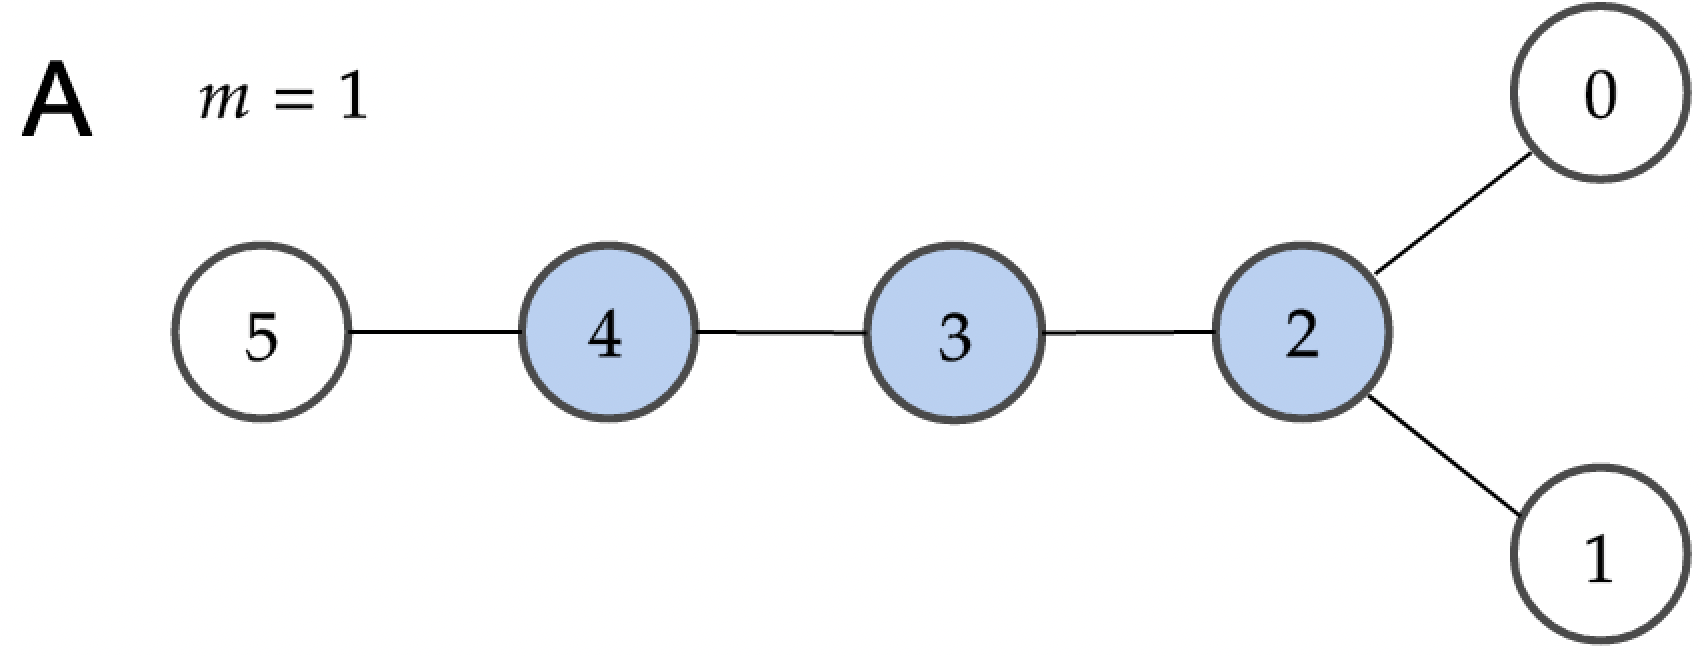
\includegraphics[width=8cm]{latex/Images/input_graph_G_6_0_alternative1.png}
%    \caption{Example input graph. For $m=1$ the algorithm still selects 3 nodes as it is an approximation of the MDS.}
%    \label{fig:input_graph}
%\end{figure}
\begin{rudifig}{\hsize}{Fig. 1: Input Graph}
    
    \hspace{-1em}
    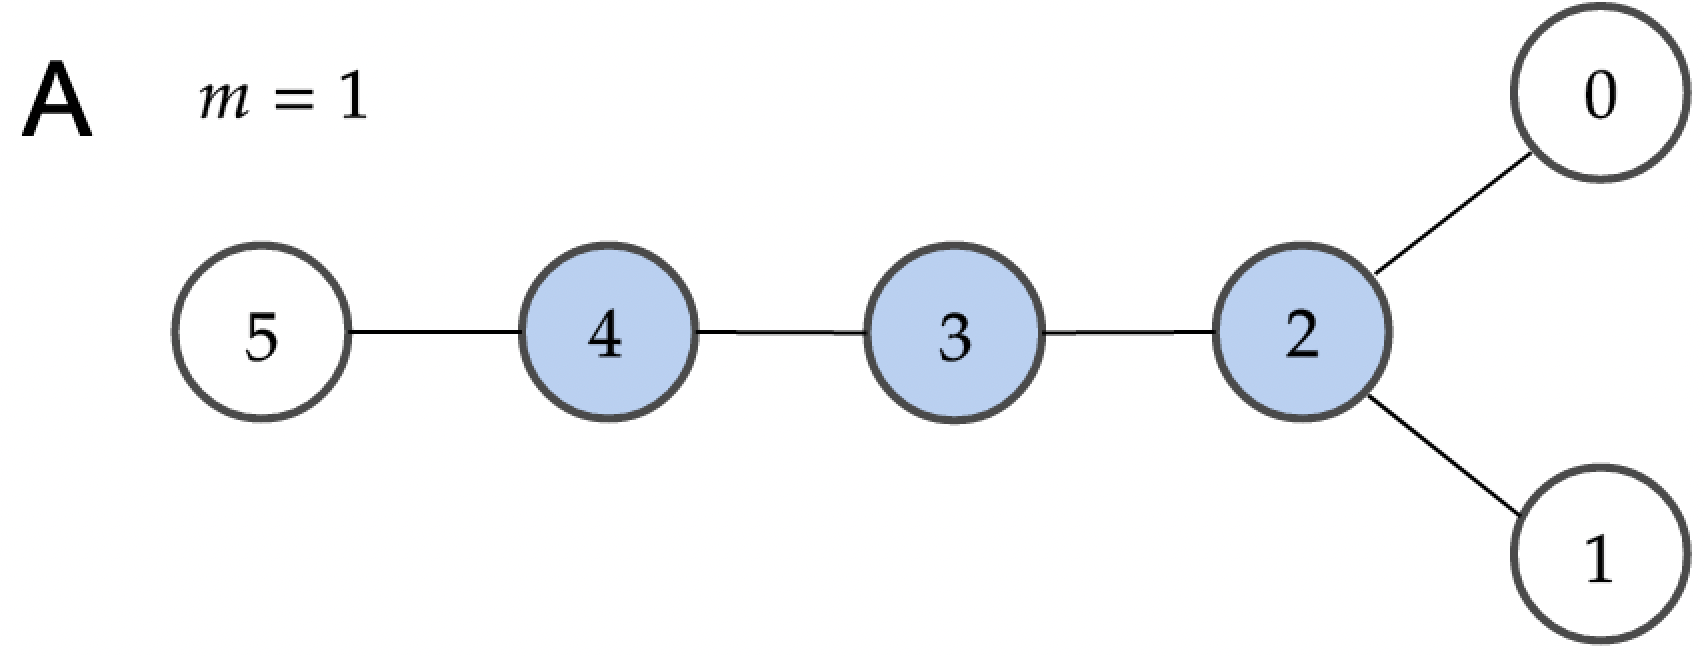
\includegraphics[width=8cm]{latex/Images/input_graph_G_6_0_alternative1.png}
    %\caption{Example input graph. For $m=1$ the algorithm still selects 3 nodes as it is an approximation of the MDS.}
    \label{fig:input_graph}
\end{rudifig}

%\begin{figure}[]
%    \centering
%    %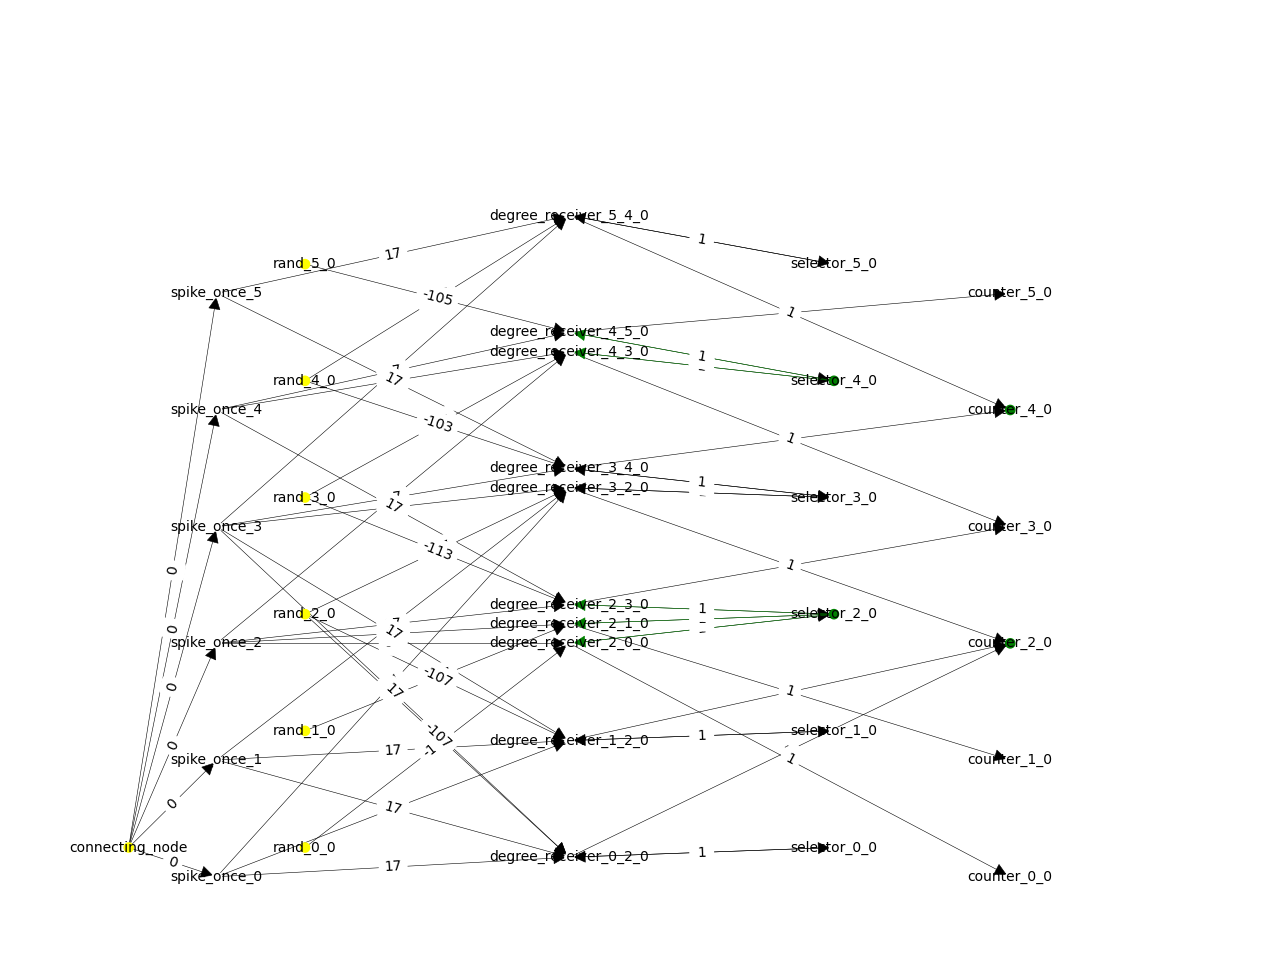
\includegraphics[width=8cm]{latex/Images/structured_graph_snn_m0_n6_iter0_t77.png}
%    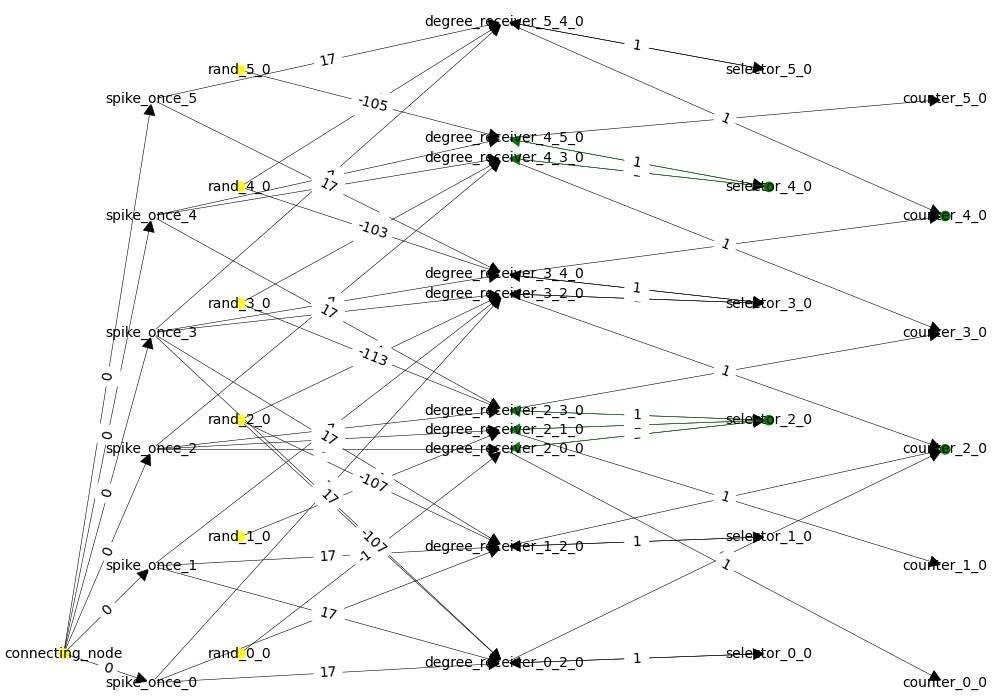
\includegraphics[width=\linewidth]{latex/Images/cropped.jpeg}
%    \caption{Example SNN encoding of algorithm to approximate MDS on the input graph of \cref{fig:input_graph}. This module is connected in series where the mark counter neuron takes up the role of spike\_once neuron in the next round of the approximation algorithm. For a more detailed description of the SNN implementation the reader is referred to Diehl et al. \cite{diehl}. %TODO: update to match updated input graph.
%    }
%    \label{fig:encoded_snn}
%\end{figure}
\begin{rudifig}{\hsize}{Fig. 2: Example SNN}
    
    \hspace{-1em}
    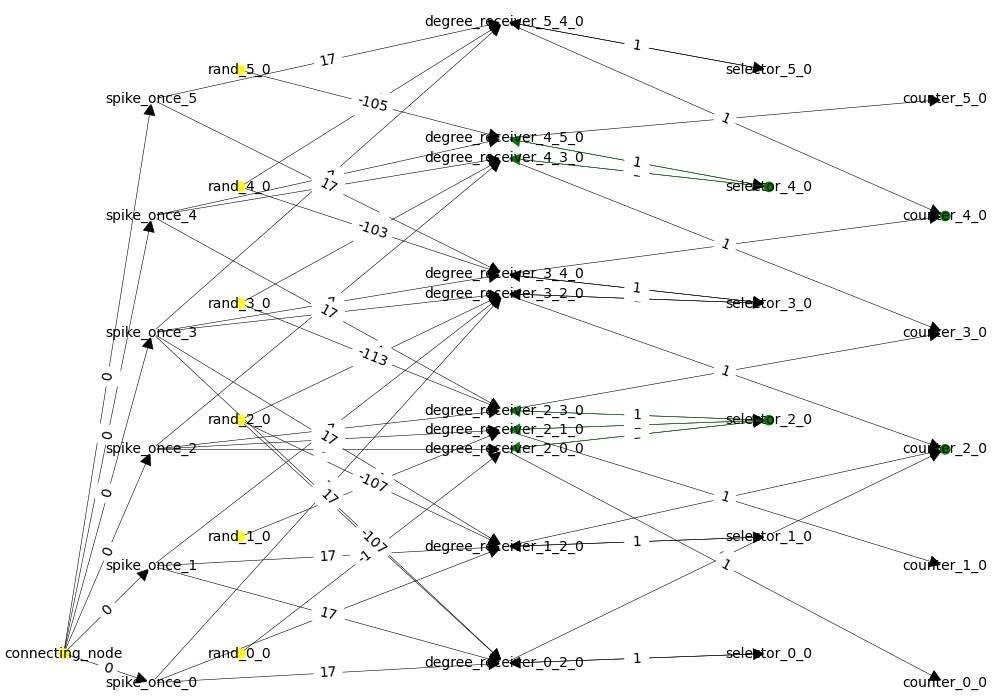
\includegraphics[width=\linewidth]{latex/Images/cropped.jpeg}
    %\caption{Example SNN encoding of algorithm to approximate MDS on the input graph of \cref{fig:input_graph}. This module is connected in series where the mark counter neuron takes up the role of spike\_once neuron in the next round of the approximation algorithm. For a more detailed description of the SNN implementation the reader is referred to Diehl et al. \cite{diehl}. %TODO: update to match updated input graph.
    %}
    \label{fig:encoded_snn}
\end{rudifig}

\noindent This SSN implementation of the MDS approximation algorithm is onwards referred to as the default network. This default network is enhanced with strategically placed redundant neurons that are inhibited by the default network neurons. Next, space radiation damage is simulated on the Loihi 2 in the form of random neuron deaths. These neuron deaths imply that a neuron is removed from the SNN, which can occur in both the default network and the set of redundancy neurons. If a default network neuron dies, the inhibition to the redundant neuron should be removed, causing the SNN to use the alternative neural pathway to recover from this damage. This usage of the alternative neural pathway simulates the multi-pathway structures found in brains of higher vertebrates and is proposed as the main adaptive mechanism in response to damage.

\subsection{Hardware}\label{subsec:hardware}
At the time of writing, no single-event effect (SEEs) propagation mechanisms are identified for space radiation exposure on the Loihi 1 \& 2  neuromorphic chips, a high-level software simulation of these single-event effects is performed. This is done by assuming that the non-neuromorphic components of the chips are performing nominally, and that the SEEs propagate from, for example, transient bit-flips, towards neuronal and synaptic parameter changes. The first assumptions may be accurate if local radiation hardening and redundancy is applied to the non-neuromorphic components. Weight and/or energy saving could be a motivation to apply these radiation counter-measures sparsely. The second assumption is based on the digital nature of the components that make up the neural components of the Loihi. %The components that make up the neural compartments and synapses of the Loihi are visualised in \cref{fig:loihi_micro_architecture}.
%\begin{figure}[H]
%    \centering
%    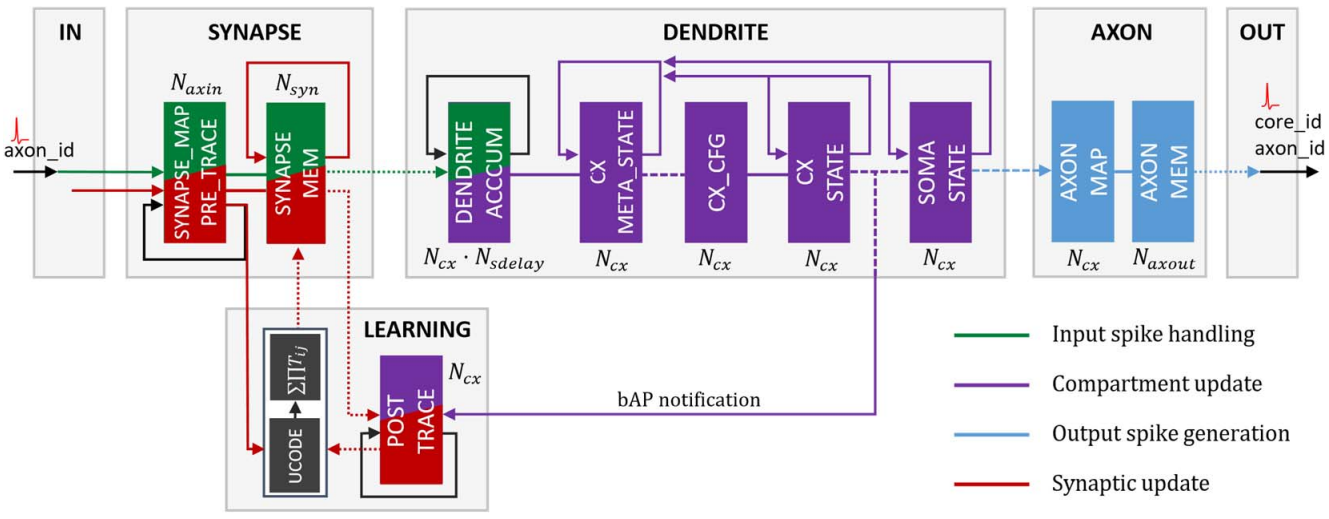
\includegraphics[width=8cm]{latex/Images/loihi_micro_architecture.png}
%    \caption{Core Top-Level Microarchitecture of the Loihi chip. The SYNAPSE unit processes all incoming spikes and
%    reads out the associated synaptic weights from the SRAM memory \cite{davies_loihi_2018}
%    .}
%    \label{fig:loihi_micro_architecture}
%\end{figure}




\subsection{Testing}\label{subsec:testing}
To test whether the brain adaptation implementation may be used to increase radiation robustness of neuromorphic space hardware, it is compared to a baseline without brain adaptation. 

% TODO: verify subsubsections are allowed.
\subsubsection{Metrics}\label{subsubsec:metrics}
The metrics of the comparison are:
\begin{enumerate}
    \item \textit{Radiation Robustness} - a percentage score indicating the ratio of successful solution generation on random input graphs.
    \item \textit{Neuronal \& Synaptic Overcapacity} - a factor from 0 to $n$, indicating the ratio of redundant neurons and synapses with respect to the original implementation without adaptation implementation. % TODO: consistent default network naming see method/intro.
    \item \textit{Energy Efficiency} - the number of spikes consumed by implementations.
    %\item \textit{Time complexity} - the theoretical time complexity required for network initialisation and adaptation.
    %\item \textit{Space Complexity} - the theoretical space complexity required for network initialisation and adaptation.
\end{enumerate}

\subsubsection{Simulated Radiation Damage}\label{subsubsec:simulated_radiation_damage}
This work simulates radiation damage propagation of SEEs as neuron deaths by setting the neuron thresholds $vth=1000 [V]$ at from the start of the simulation. The 1000 [V] is arbitrary yet large enough to prevent spiking. Transient effects are ignored along with neuron property changes in $\delta u,\delta v, bias$, synaptic death, and synaptic property changes in: $sign,weight$.

\subsubsection{Brain Adaptation Mechanism}\label{subsubsec:brain_adaptation_mechanisms}
The selected SNN implementation is enhanced with redundant neurons and neuronal pathways to realise simulated radiation robustness. A basic example is shown in \cref{fig:eg_brain_adaptation}.
% Non poster image:
%\begin{figure}[H]
%    \centering
%    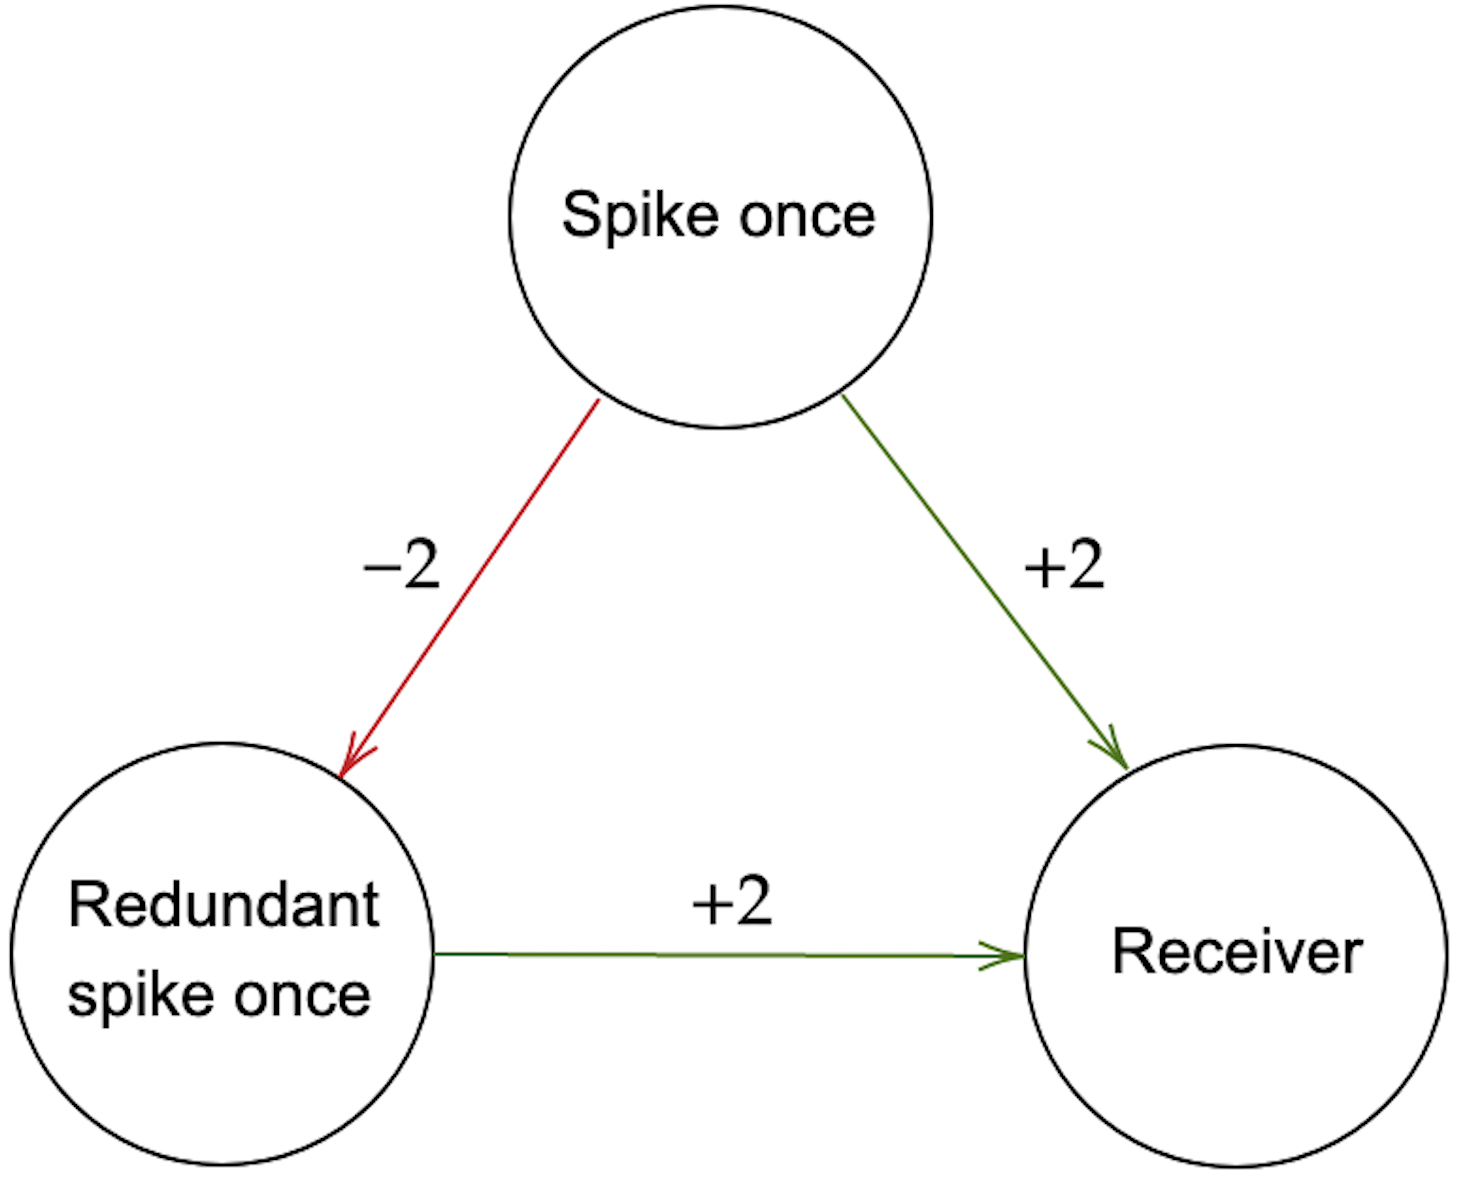
\includegraphics[width=.5\linewidth]{latex/Images/brain_adaptation_alternative.png}
%    \caption{Alternative neural pathway for a redundancy of the spike\_once neuron. If the spike\_once neuron dies due to simulated radiation-induced SEEs ($vth=inf$), the redundancy neuron inhibition is eliminated. Without inhibition, the redundant spike\_once neuron copies the spike\_once behaviour with a delay of 1 timestep.}
%    \label{fig:eg_brain_adaptation}
%\end{figure}
\begin{rudifig}{\hsize}{Fig. 3: Redundancy}
    %
\includegraphics[width=\hsize]{ru_en_1}
    \hspace{-1em}
    %
\includegraphics[width=700pt]{latex/Images/os0.jpg}
    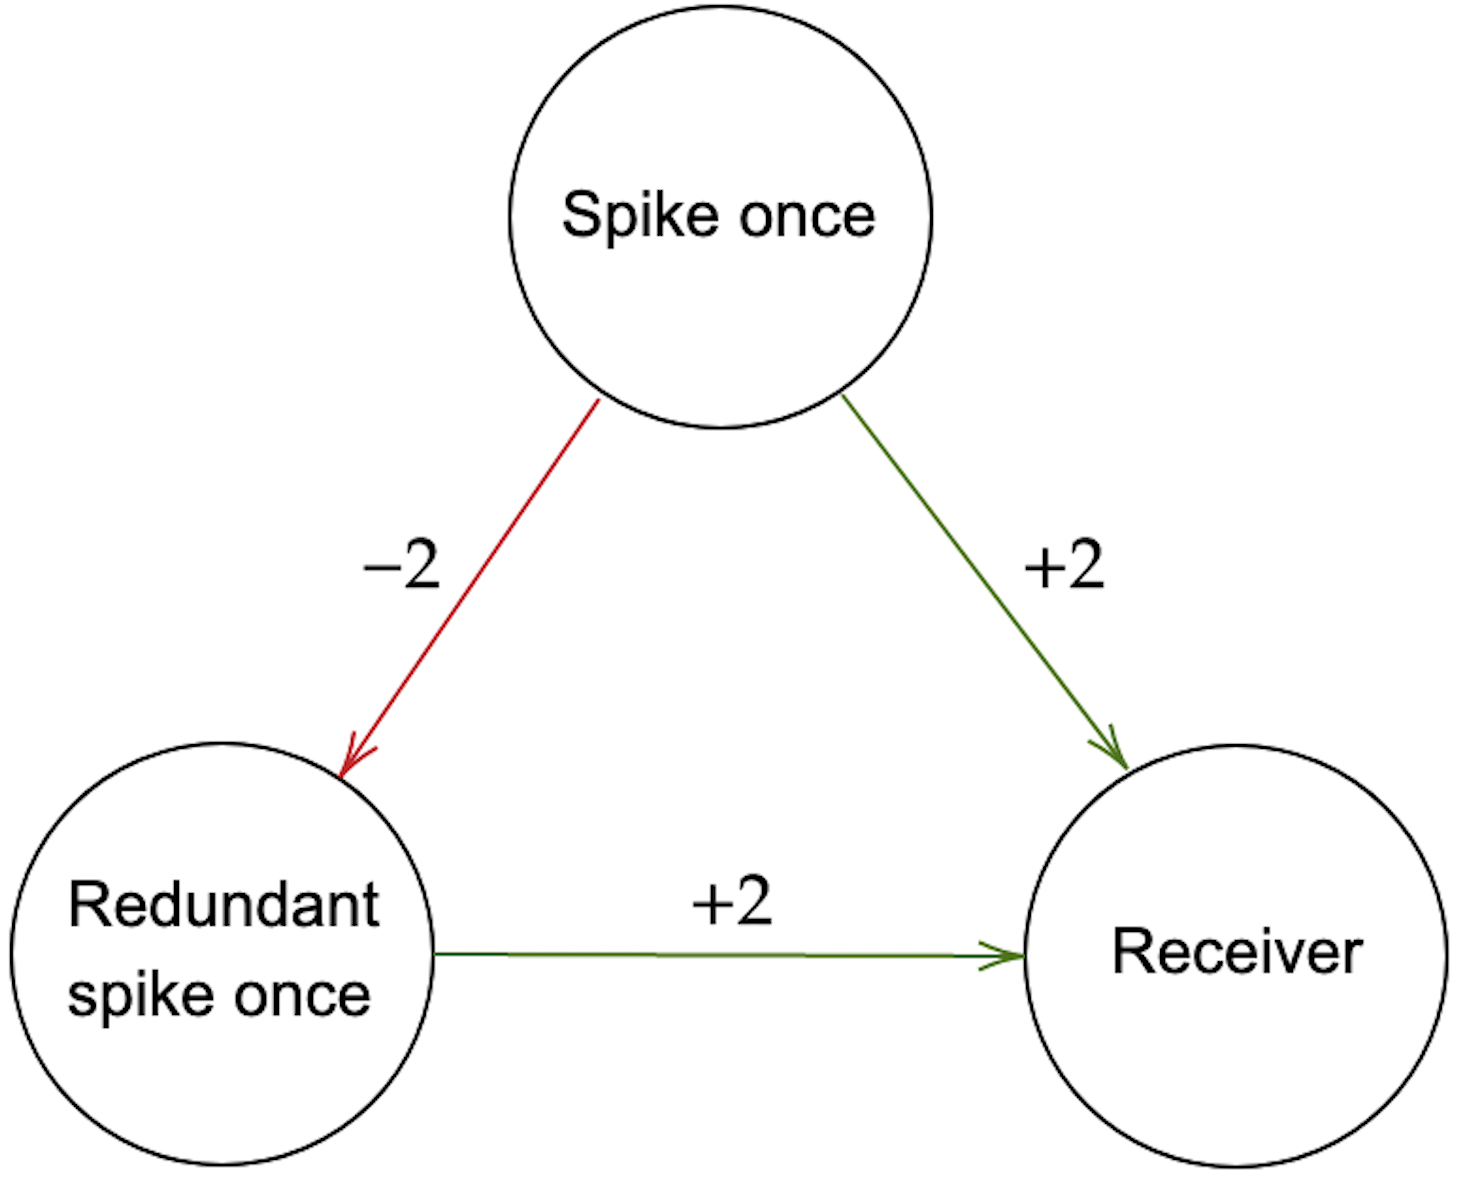
\includegraphics[width=700pt]{latex/Images/brain_adaptation_alternative.png}
    %\caption{Alternative neural pathway for a redundancy of the spike\_once neuron. If the spike\_once neuron dies due to simulated radiation-induced SEEs ($vth=inf$), the redundancy neuron inhibition is eliminated. Without inhibition, the redundant spike\_once neuron copies the spike\_once behaviour with a delay of 1 timestep.}
    \label{fig:eg_brain_adaptation}
\end{rudifig}


\noindent The alternative neural pathway renders a single neuron $original_i$ with $a$ input synapses, and $b$ output synapses, redundant at the cost of $2a+2b$ synapses and 2 neurons. This cost can be reduced by implementing a controller that scans the network and manually redirects neural pathways to a smaller buffer network. However, that shifts the radiation robustness problem as that controller may also endure SEEs. % This does allow local shielding to be used, and may use components that are physically more robust than the SNN networks.
One can also add triple/$n$-factor redundancy by including more redundant spike\_once neurons that are inhibited by the original spike\_once neuron and each other. This induces an additional delay of t=1 time step per redundant neuron.

%\item \textcolor{red}{An Neumann monitoring module that scans the entire SNN network probing its behaviour, and re-routing broken neurons and/or synapses to redundant neurons.}
%\item \textcolor{red}{A rate-coding frequency adaptation to reduce the relative impact of radiation induced spike omission in a subnetwork of the complete SNN implementation of the MDS approximation.}

        \else
            % Local compilation
            \section{Methodology}\label{sec:methodology}
The research methodology starts in \cref{subsec:algorithm} with a description of the minimum dominating set (MDS) approximation algorithm by Alipour, the SNN implementation of this algorithm by Diehl et al., and the implemented form %TODO: form or forms? 
of brain adaptation \cite{alipour2020distributed}\cite{diehl}. Since the overarching research project aims at performing physical radiation tests, \cref{subsec:hardware} specifies the hardware that is used for testing, and how the radiation effects are simulated. The test procedure is detailed in \cref{subsec:testing}.

\subsection{Algorithm Selection}\label{subsec:algorithm}
The MDS approximation as presented by Alipour et al., is specified in Alg. 1.
%Within the graph algorithms, some SNN algorithms may be naturally more robust than others. For example, SNN algorithms that calculate the shortest path within graphs may automatically re-route if radiation imposed neuron-death occurs. However, since this research aims at determining the effectivity of brain adaptation mechanisms, a stricter test is found in algorithms that can fail to produce meaningful output if a single neuronal or synaptic property is changed. Therefore, 
%%%\begin{algorithm}[h]%[1]
%%%    \caption{Distributed Algorithm for computing a total dominating set in a graph with given integer $m\geq 0$.}\label{alg:alipour}
%%%    \KwData{Connected, planar, triangle-free graph of size $n$.}
%%%    \KwResult{Set of nodes that form a minimum total dominating set (MDTS).}
%%%    In the first round, each node $v_i$ chooses a random number $0<r_i<1$ and computes its weight $w_i=d_i+r_i$ and sends $w_i$ to its
%%%    adjacent neighbours.\;
%%%    In the second round, each node $v$ marks a neighbour vertex $v_i$ whose weight $w_i$ is maximum among all the other neighbours of $v$.\;
%%%    \For{$m$ rounds}{
%%%        Let $x_i$ be the number of times that a vertex is marked by its neighbour vertices, let $w_i=x_i+r_i$\;
%%%        Unmark the marked vertices.\;
%%%        Each vertex marks the vertex with maximum $w_i$ among its neighbour vertices.\;
%%%    }
%%%    8: The marked vertices are considered as the vertices in our total dominating set for $G$.\;
%%%\end{algorithm}
Next, an SNN implementation of this algorithm is generated using Leaky-Integrate-and-Fire (LIF) neurons. This implementation is created by Diehl et al. \cite{diehl} using the open-source Lava software framework by Intel. This implementation takes as input connected, triangle-free, planar graphs (E.g. \cref{fig:input_graph}). Then it converts these graphs into the specification of an SNN that is encoded in a new graph (E.g. \cref{fig:encoded_snn}). A recursive method then takes a single neuron and converts the encoded SNN that is encoded in the graph into an actual functional SNN that can be run on the simulated on a regular computer.
%\begin{figure}[]
%    \centering
%    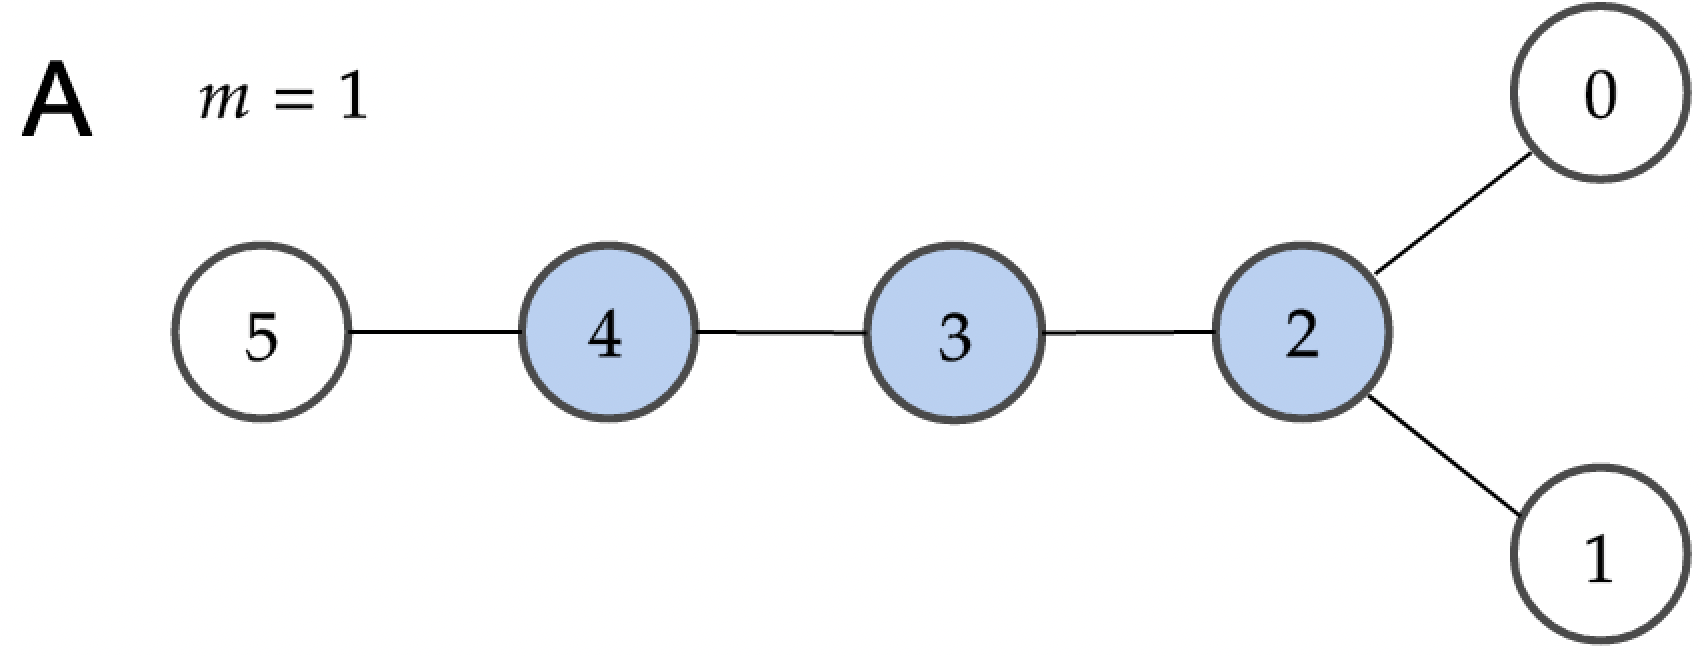
\includegraphics[width=8cm]{latex/Images/input_graph_G_6_0_alternative1.png}
%    \caption{Example input graph. For $m=1$ the algorithm still selects 3 nodes as it is an approximation of the MDS.}
%    \label{fig:input_graph}
%\end{figure}
\begin{rudifig}{\hsize}{Fig. 1: Input Graph}
    
    \hspace{-1em}
    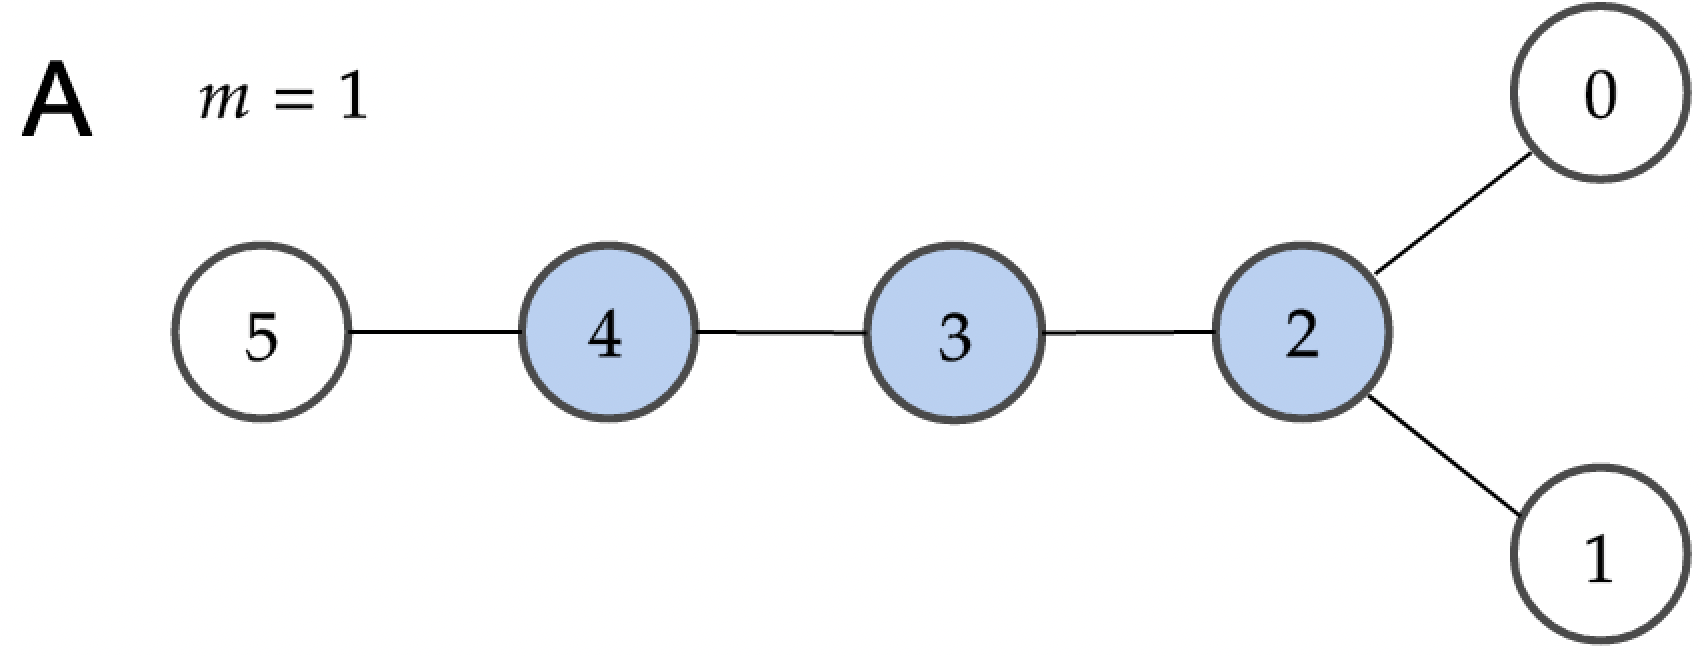
\includegraphics[width=8cm]{latex/Images/input_graph_G_6_0_alternative1.png}
    %\caption{Example input graph. For $m=1$ the algorithm still selects 3 nodes as it is an approximation of the MDS.}
    \label{fig:input_graph}
\end{rudifig}

%\begin{figure}[]
%    \centering
%    %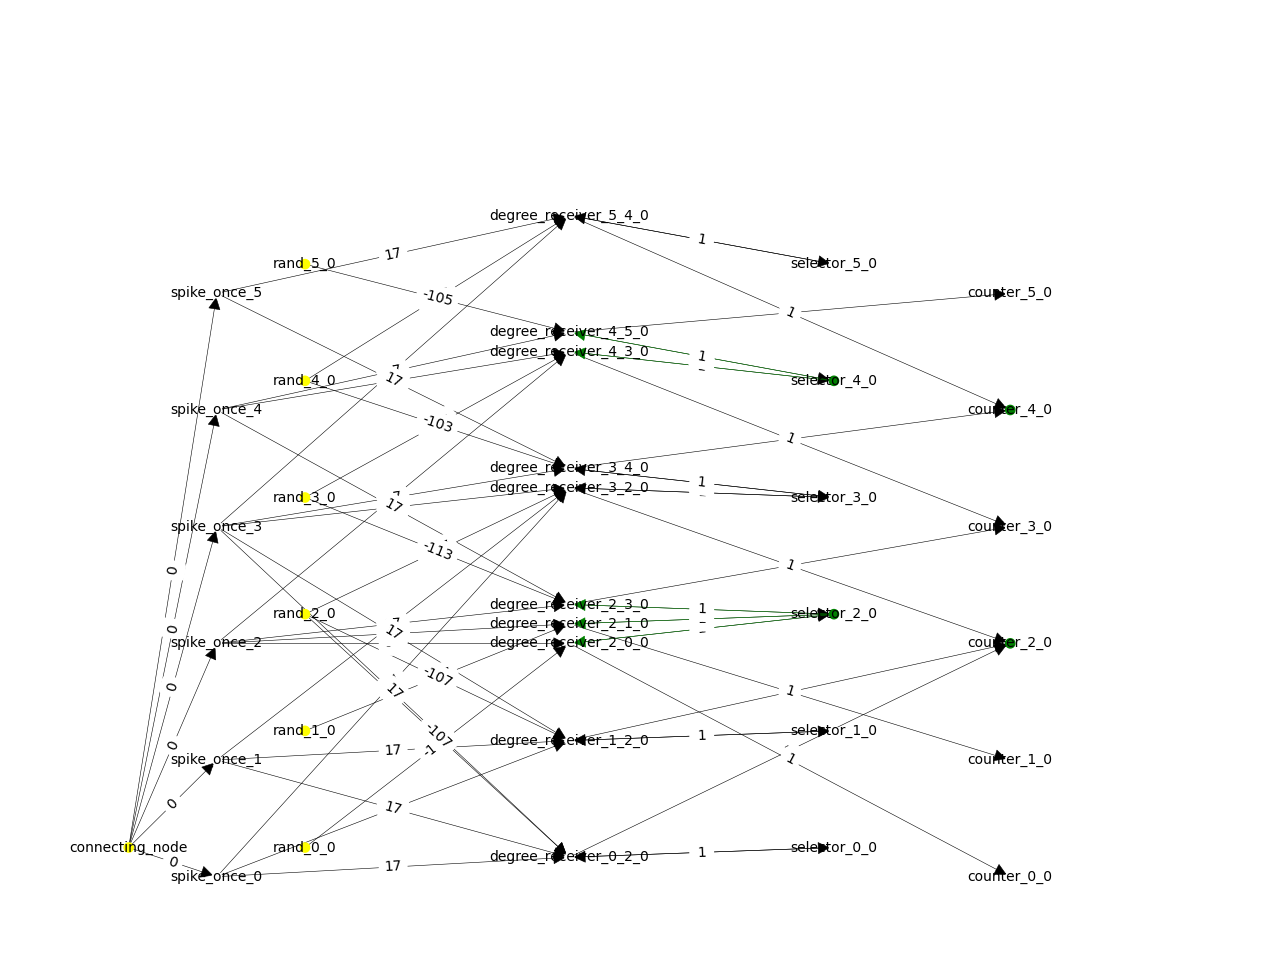
\includegraphics[width=8cm]{latex/Images/structured_graph_snn_m0_n6_iter0_t77.png}
%    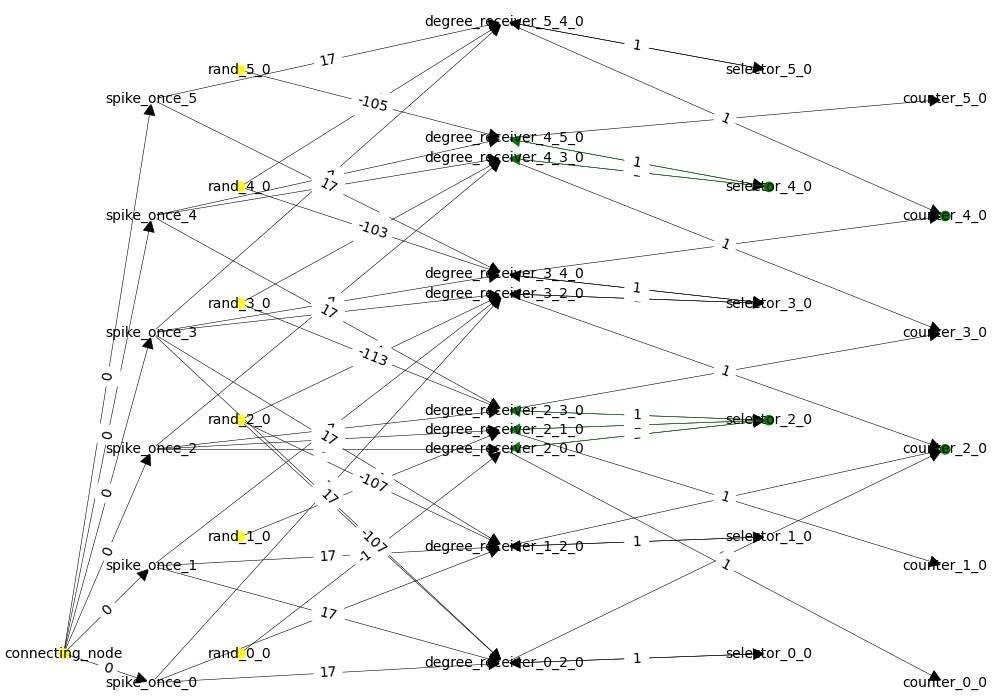
\includegraphics[width=\linewidth]{latex/Images/cropped.jpeg}
%    \caption{Example SNN encoding of algorithm to approximate MDS on the input graph of \cref{fig:input_graph}. This module is connected in series where the mark counter neuron takes up the role of spike\_once neuron in the next round of the approximation algorithm. For a more detailed description of the SNN implementation the reader is referred to Diehl et al. \cite{diehl}. %TODO: update to match updated input graph.
%    }
%    \label{fig:encoded_snn}
%\end{figure}
\begin{rudifig}{\hsize}{Fig. 2: Example SNN}
    
    \hspace{-1em}
    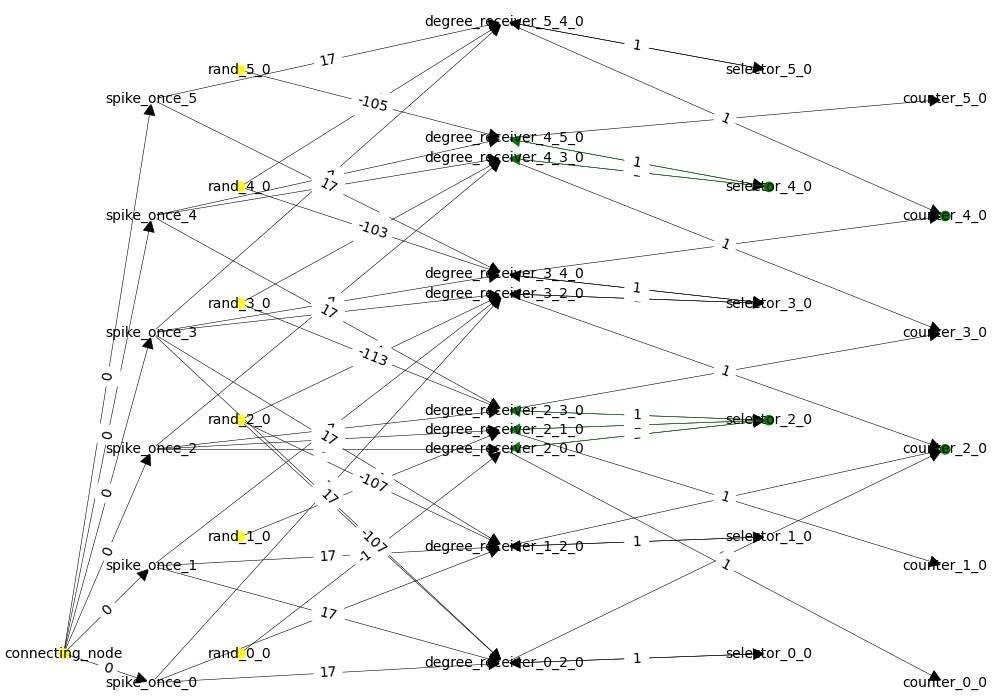
\includegraphics[width=\linewidth]{latex/Images/cropped.jpeg}
    %\caption{Example SNN encoding of algorithm to approximate MDS on the input graph of \cref{fig:input_graph}. This module is connected in series where the mark counter neuron takes up the role of spike\_once neuron in the next round of the approximation algorithm. For a more detailed description of the SNN implementation the reader is referred to Diehl et al. \cite{diehl}. %TODO: update to match updated input graph.
    %}
    \label{fig:encoded_snn}
\end{rudifig}

\noindent This SSN implementation of the MDS approximation algorithm is onwards referred to as the default network. This default network is enhanced with strategically placed redundant neurons that are inhibited by the default network neurons. Next, space radiation damage is simulated on the Loihi 2 in the form of random neuron deaths. These neuron deaths imply that a neuron is removed from the SNN, which can occur in both the default network and the set of redundancy neurons. If a default network neuron dies, the inhibition to the redundant neuron should be removed, causing the SNN to use the alternative neural pathway to recover from this damage. This usage of the alternative neural pathway simulates the multi-pathway structures found in brains of higher vertebrates and is proposed as the main adaptive mechanism in response to damage.

\subsection{Hardware}\label{subsec:hardware}
At the time of writing, no single-event effect (SEEs) propagation mechanisms are identified for space radiation exposure on the Loihi 1 \& 2  neuromorphic chips, a high-level software simulation of these single-event effects is performed. This is done by assuming that the non-neuromorphic components of the chips are performing nominally, and that the SEEs propagate from, for example, transient bit-flips, towards neuronal and synaptic parameter changes. The first assumptions may be accurate if local radiation hardening and redundancy is applied to the non-neuromorphic components. Weight and/or energy saving could be a motivation to apply these radiation counter-measures sparsely. The second assumption is based on the digital nature of the components that make up the neural components of the Loihi. %The components that make up the neural compartments and synapses of the Loihi are visualised in \cref{fig:loihi_micro_architecture}.
%\begin{figure}[H]
%    \centering
%    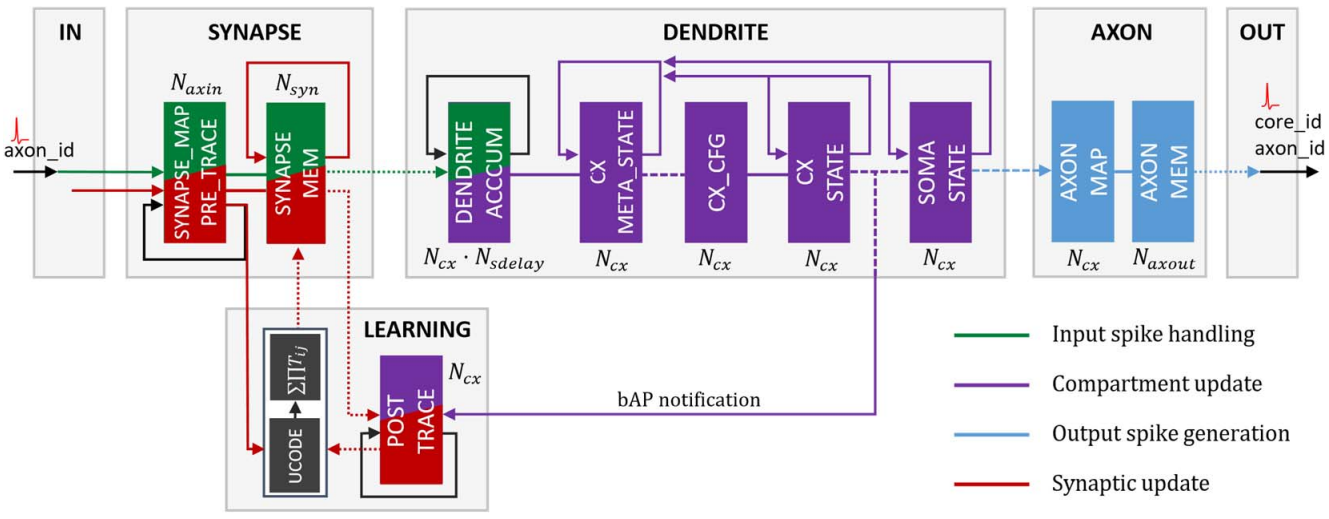
\includegraphics[width=8cm]{latex/Images/loihi_micro_architecture.png}
%    \caption{Core Top-Level Microarchitecture of the Loihi chip. The SYNAPSE unit processes all incoming spikes and
%    reads out the associated synaptic weights from the SRAM memory \cite{davies_loihi_2018}
%    .}
%    \label{fig:loihi_micro_architecture}
%\end{figure}




\subsection{Testing}\label{subsec:testing}
To test whether the brain adaptation implementation may be used to increase radiation robustness of neuromorphic space hardware, it is compared to a baseline without brain adaptation. 

% TODO: verify subsubsections are allowed.
\subsubsection{Metrics}\label{subsubsec:metrics}
The metrics of the comparison are:
\begin{enumerate}
    \item \textit{Radiation Robustness} - a percentage score indicating the ratio of successful solution generation on random input graphs.
    \item \textit{Neuronal \& Synaptic Overcapacity} - a factor from 0 to $n$, indicating the ratio of redundant neurons and synapses with respect to the original implementation without adaptation implementation. % TODO: consistent default network naming see method/intro.
    \item \textit{Energy Efficiency} - the number of spikes consumed by implementations.
    %\item \textit{Time complexity} - the theoretical time complexity required for network initialisation and adaptation.
    %\item \textit{Space Complexity} - the theoretical space complexity required for network initialisation and adaptation.
\end{enumerate}

\subsubsection{Simulated Radiation Damage}\label{subsubsec:simulated_radiation_damage}
This work simulates radiation damage propagation of SEEs as neuron deaths by setting the neuron thresholds $vth=1000 [V]$ at from the start of the simulation. The 1000 [V] is arbitrary yet large enough to prevent spiking. Transient effects are ignored along with neuron property changes in $\delta u,\delta v, bias$, synaptic death, and synaptic property changes in: $sign,weight$.

\subsubsection{Brain Adaptation Mechanism}\label{subsubsec:brain_adaptation_mechanisms}
The selected SNN implementation is enhanced with redundant neurons and neuronal pathways to realise simulated radiation robustness. A basic example is shown in \cref{fig:eg_brain_adaptation}.
% Non poster image:
%\begin{figure}[H]
%    \centering
%    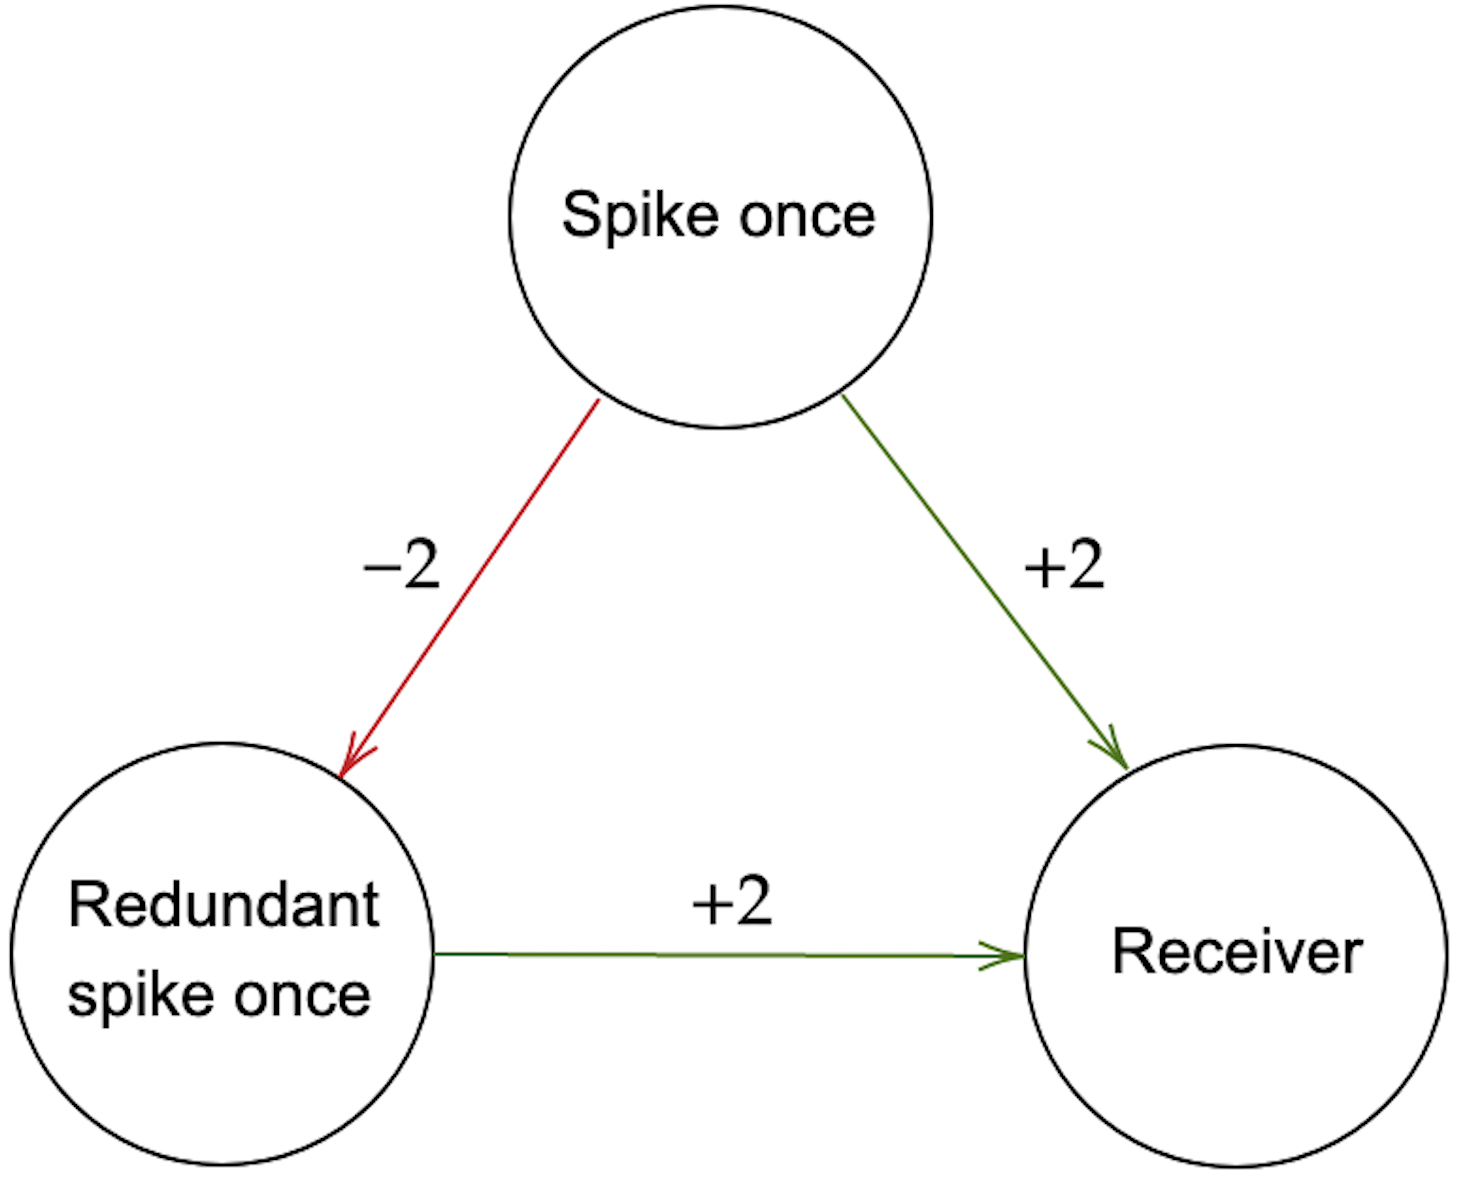
\includegraphics[width=.5\linewidth]{latex/Images/brain_adaptation_alternative.png}
%    \caption{Alternative neural pathway for a redundancy of the spike\_once neuron. If the spike\_once neuron dies due to simulated radiation-induced SEEs ($vth=inf$), the redundancy neuron inhibition is eliminated. Without inhibition, the redundant spike\_once neuron copies the spike\_once behaviour with a delay of 1 timestep.}
%    \label{fig:eg_brain_adaptation}
%\end{figure}
\begin{rudifig}{\hsize}{Fig. 3: Redundancy}
    %
\includegraphics[width=\hsize]{ru_en_1}
    \hspace{-1em}
    %
\includegraphics[width=700pt]{latex/Images/os0.jpg}
    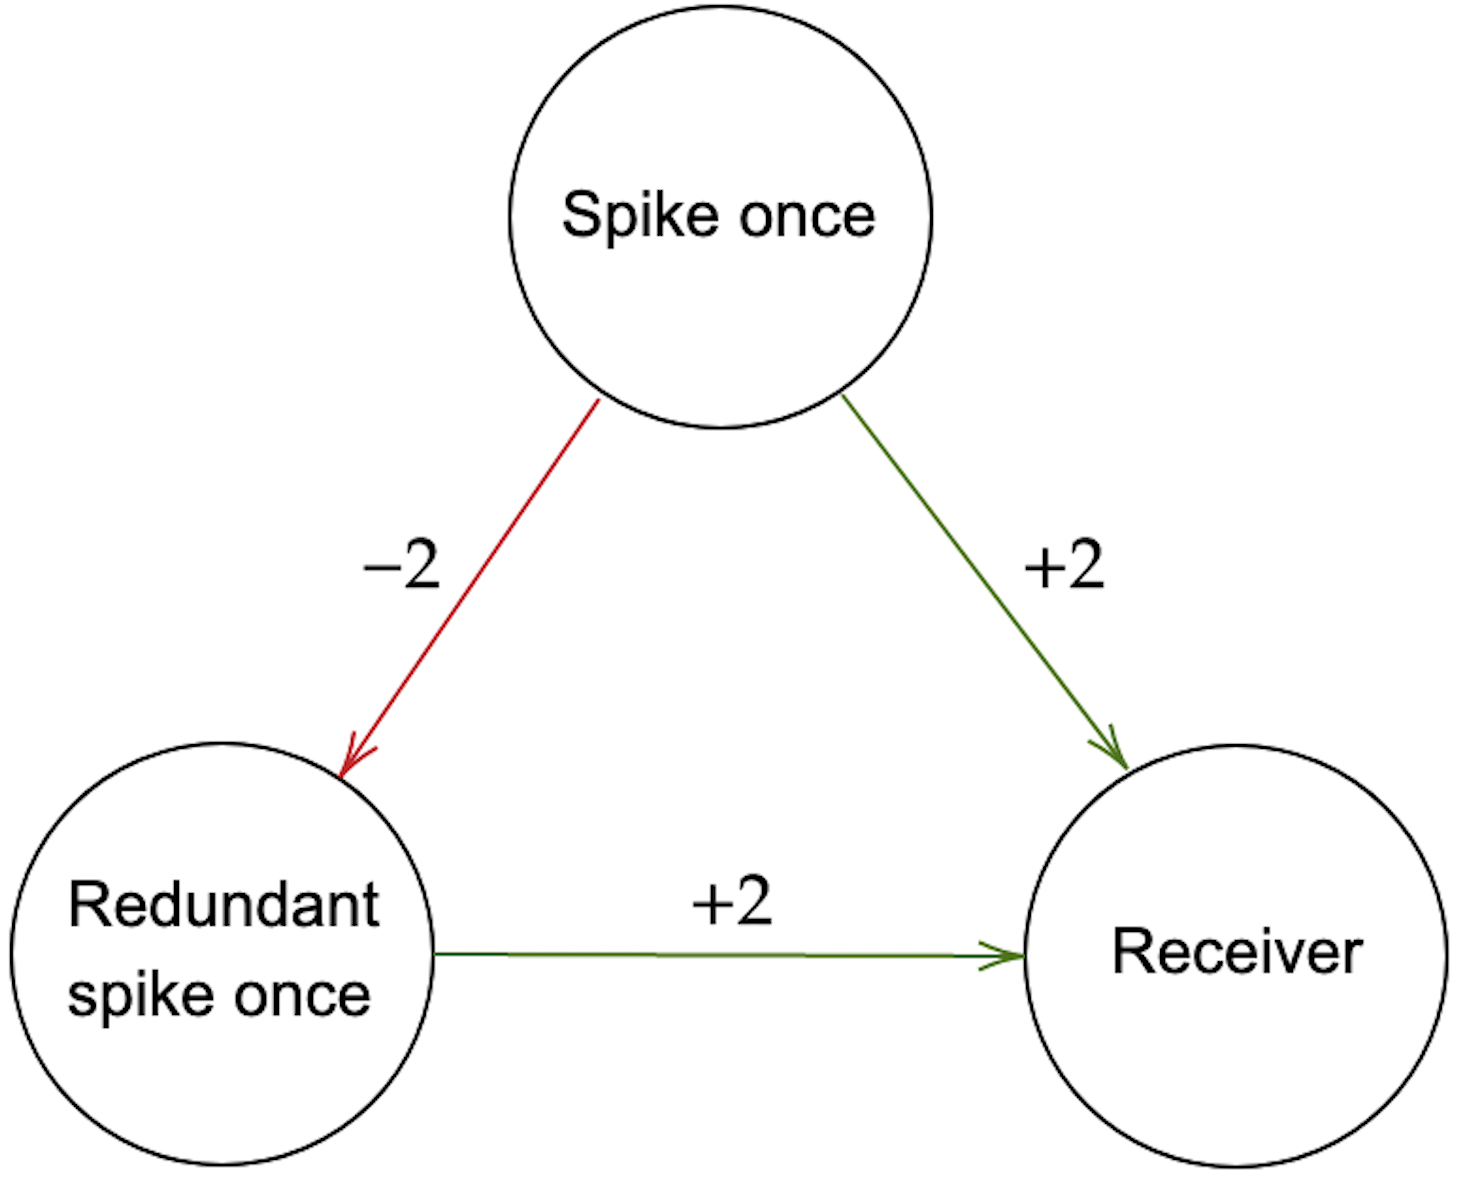
\includegraphics[width=700pt]{latex/Images/brain_adaptation_alternative.png}
    %\caption{Alternative neural pathway for a redundancy of the spike\_once neuron. If the spike\_once neuron dies due to simulated radiation-induced SEEs ($vth=inf$), the redundancy neuron inhibition is eliminated. Without inhibition, the redundant spike\_once neuron copies the spike\_once behaviour with a delay of 1 timestep.}
    \label{fig:eg_brain_adaptation}
\end{rudifig}


\noindent The alternative neural pathway renders a single neuron $original_i$ with $a$ input synapses, and $b$ output synapses, redundant at the cost of $2a+2b$ synapses and 2 neurons. This cost can be reduced by implementing a controller that scans the network and manually redirects neural pathways to a smaller buffer network. However, that shifts the radiation robustness problem as that controller may also endure SEEs. % This does allow local shielding to be used, and may use components that are physically more robust than the SNN networks.
One can also add triple/$n$-factor redundancy by including more redundant spike\_once neurons that are inhibited by the original spike\_once neuron and each other. This induces an additional delay of t=1 time step per redundant neuron.

%\item \textcolor{red}{An Neumann monitoring module that scans the entire SNN network probing its behaviour, and re-routing broken neurons and/or synapses to redundant neurons.}
%\item \textcolor{red}{A rate-coding frequency adaptation to reduce the relative impact of radiation induced spike omission in a subnetwork of the complete SNN implementation of the MDS approximation.}

        \fi

    \end{multicols}
\end{rudiblockiintroduction}

%%\begin{rudiblockimethodsresultsbody}
%%    \begin{multicols}{3}
%%    Instead of competing with each other, open source software could enable cooperation between airlines to facilitate for example the development of logistics platforms to facilitate electric or hydrogen aircrafts. This could be an example, where a collaborative development could lead to an alleviation of CO2 emission burdens on the KLM whilst boosting the aviation industry in its entirety.
%%    
%%    In other words, by adopting to an open source business model, KLM can contribute to society and connect with society in synergy. The investments in the development of open source software can be reciprocated by enabling the community to build upon and enhance the software of KLM, yielding new and innovative insights as illustrated in the included figure. Furthermore it boosts related economic activity as well as sustainability. To illustrate this, 
%%    
%%    \indent Another potential benefit of COSS is the opportunity for other businesses to add value to your business. For example, open source energy management software could enable new pioneering companies such as the local green energy company Vandebron to integrate the part of the (future) electric fleet of KLM undergoing maintenance, with their electric car network balancing grid. This way aircraft maintenance costs could be reduced by re-purposing assets through open source software. The main takeaway here is that COSS enables enhancement of the KLM assests, markets and innovation by diversifying the applicability of their development efforts through open source.
%%
%%    \indent Furthermore, open source software is required to be able to verify the security of the software. Without the ability to verify what is written in the source code, organisations cannot be absolutely certain what the degree of security of the software is. To illustrate how critical this security is becoming in an era where economic state sponsored espionage occurs increasingly more frequently, one only has to look at our neighbours at the other side of the channel where the head of MI5 Jonathan Evans confirmed a UK company lost 800 million pounds in a state sponsored espionage affair. By opening up your source code you are exposing it directly to any potential adversaries makes it easier to find any weaknesses in your code and at the same time, you enable millions of developers world wide to perform security audits to identify weaknesses in your code such that the security leaks can be discovered and patched. 
%%    
%%    \indent Illustrating the financial attractiveness of COSS is perhaps best done by looking at the acquisition of open source company Red Hat by IBM for 34 billion dollars. This follows a trend of cutting edge tech companies such as Tesla, Docker, Netflix and Spotify, to transform towards- and expand a position as an open source company. This effect of contributing to the society enhances participation of KLM in the public domain, which can be reciprocated by an attraction of the tech-industry top talent. This is illustrated by the difficulties that the top financial institutes face in attracting the technical top talents whilst competing with Silicon Valley in this market.
%%    
%%    \begin{rudifig}{\hsize}{Fig. 1: Open Source Enhancing Ideation}
%%        %
\includegraphics[width=\hsize]{ru_en_1}
%%        \hspace{-1em}
%%        
\includegraphics[width=700pt]{latex/Images/os0.jpg}
%%        %\caption{test}\label{fig:open_source}
%%    \end{rudifig}
%%    \end{multicols}
%%% 	base: \the\rudisizebase\par
%%%     paperheight: \the\paperheight\par
%%%     paperwidth: \the\paperwidth\par
%%%     header: \the\rudisizeblockheader\par
%%%     intro: \the\rudisizeblockintro\par 
%%%     methods: \the\rudisizeblockmethodsresultsbody\par 
%%%     results: \the\rudisizeblockresults\par 
%%%     discussion: \the\rudisizeblockdiscussion\par 
%%%     margin: \the\rudisizemargin\par 
%%%     $\int_0^{2\pi}\sin(x)dx=0$
%%%     $$\int_0^{2\pi}\cos(x)dx=0$$
%%    
%%    % subsection in main
%%    \begin{rudisubblock}{\hsize}{Increasing Asset Evaluation Accuracy}
%%    	Currently KLM uses the straight line method for the amortisation of software to keep track of the devaluation of the value of the software products they have produced over time [2]. When switching to COSS, a larger fraction of the KLM assets will consist of software, hence to be able to maintain an accurate asset value analyis, the straight line method can be replaced by a dedicated software valuation model for software as provided by M. Ben-Menachem and I. Gavious[1].
%%    \end{rudisubblock}
%%\end{rudiblockimethodsresultsbody}

% ======================================================================

\begin{rudiblockconclusion}
    \begin{multicols}{3}
        %KLM could turn this crisis into an opportunity to nimbly redirect its workforce towards an open source business model. The KLM Transformation Team can facilitate this transition to truly enhance its Customer Experience, Inflight Service, Information Services, Human Resources \& Industrial Relations and Corporate Center Teams. 
        The KLM Transformation Team can turn the challenging conditions into an opportunity by transitioning to a COSS business model.
        
        KLM can amplify its integrated position in the transport industry with the adoption of a company-wide COSS business model and enable other companies to diversify and extend the KLM software. This can lead to new innovative solutions by fresh eyes looking at the same challenges that KLM currently faces.
        
        While COSS allows adversaries to read source code, it also enables millions of developers access which ensures bugs and security risks can be identified and solved quicker than with closed source development[4]. COSS is the only way for third parties to know the code is safe as they cannot verify the security of proprietary software[4].
        
        Furthermore, a transformation to a COSS business model enables KLM to attract top tech talent.
        
        
    \end{multicols}
\end{rudiblockconclusion}

% ======================================================================

\begin{paralleltwoblocks}{0.67}
    \begin{rudiblockipolicyrecommendations}
        \begin{multicols}{2}
            To facilitate a smooth transformation towards a COSS business model the following policy recommendations are included:
            \begin{itemize}
                \item Apply the temporary reduction of workforce size to nimbly convert KLM towards an COSS business model, incorporate the COSS business model in the hiring strategy when KLM is able to expand again and hire an additional cyber security-, data analytics- and legal team to ensure a safe transition from proprietary codebase to open source codebase.
                \item Design the COSS to set up open application programmable interfaces (APIs) in cooperation with the open source community to enable companies and community to interact with KLM through the APIs.
                \item Convert the annual amortisation method of software assets in KLM from the straight line method to the dedicated software valuation model for software as provided by M. Ben-Menachem and I. Gavious [1].
            \end{itemize}
            These three steps enable KLM to pivot to a COSS business model to successfully navigate the challenges of the early 21st century and reaffirm its pioneering position.
        \end{multicols}
    \end{rudiblockipolicyrecommendations}
    &
    {
    \begin{rudiblockaddendum}
    	\small
    	\References\par
        \Acknowledgments\par
        %\Funding
        % \url{https://www.zdnet.com/article/microsoft-dropped-for-open-source-why-hamburg-is-now-following-munichs-lead/}
        % \url{https://www.zdnet.com/article/open-source-giant-red-hat-has-a-new-ceo/}
        % \url{https://opensource.google/docs/why/}
        % \url{https://www.sciencedirect.com/science/article/abs/pii/S0268401219309867}
        % \url{https://pubsonline.informs.org/doi/abs/10.1287/deca.2019.0390}
        % \url{https://dl.acm.org/doi/fullHtml/10.1145/1188913.1188921}
        % \url{https://ieeexplore.ieee.org/abstract/document/951496}
        % \url{https://www.sciencedirect.com/science/article/pii/S0167404802005163}
        % \url{https://dl.acm.org/doi/abs/10.1145/1529282.1529731}
        
        % % Regulations
        % \url{https://journals.sagepub.com/doi/abs/10.1177/1043986219890194}
        % \url{https://iopscience.iop.org/article/10.1088/1755-1315/428/1/012098/meta}
        % \url{https://journals.sagepub.com/doi/full/10.1177/1043986219890202}
        % \url{https://link.springer.com/article/10.1057/s41284-019-00195-5}
        % \url{https://meridian.allenpress.com/jis/article-abstract/21/2/117/75564} % downward bias in the value of software
        % \url{https://www.klm.com/travel/nl_en/Images/KLM-Jaarverslag-2019_tcm542-1063986.pdf} 2019 Jaarverslag klm straight line method
    \end{rudiblockaddendum}
    }
\end{paralleltwoblocks}

% ======================================================================
% force removal of empty page at the end
% (this will not work inside `\AtEndDocument`)
\clearpage
\end{document}

